\section{Regresión Lineal}
La regresión lineal es el punto de entrada más sencillo de entender y aplicar en la Ciencia de Datos. Parte de esto se debe a que la regresión lineal es aplicable en muchos casos a una gran gama de problemas de predicción en los cuales el científico de datos cuenta con una base de datos o juego de datos lo suficientemente grande y accesible para entrenar un modelo \cite{daroczi}. La segunda razón es que un modelo bien entrenado de regresión lineal por lo general nos da una respuesta con cierto grado de precisión que da por cerrado el caso \cite{leek}.

El concepto en sí es relativamente sencillo de abstraer y explicar. En una visualización de datos donde un valor $y$ se corresponde con alguna relación del valor $x$, para cada $x$ y $y$, es posible trazar una línea que en cierta forma sea representativa del valor de predicción de $y$ para cada $x$. Esta línea puede no ser perfecta, o puede dejar muchos puntos sin una relación válida (a menos en el papel de gráfico) pero nos da una idea aproximada de la tendencia y evolución de los datos. \\

\begin{figure}[h!]
    \centering
    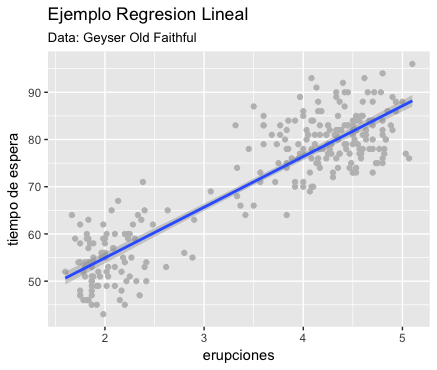
\includegraphics[width = 4 in]{ejemRegresionLineal.png}
    \caption{Ejemplo de Regresión Lineal con Old Geyser}
\end{figure}

Zumel y Mount describen la regresión lineal como el más común de los métodos de aprendizaje automatizado \cite{zumelMount}. Para los autores hay una probabilidad muy grande que el método funcione bien con el problema, y si no, es muy fácil verificar cual otro método probar como segunda opción. Para Daroczi, el énfasis está en los modelos de regresión multivariable (una extensión de la regresión lineal simple de un solo predictor y resultado) que construyen el camino para la predicción de fenómenos complejos en la naturaleza y negocios \cite{daroczi}. Por su parte, Harrington resume los beneficios de la regresión lineal \cite{harrington} por la facilidad de interpretar los resultados y lo frugal en el uso de ciclos de computación (aunque puede ser menos útil si el fenómeno no es perfectamente lineal).

\subsection{Definición de Regresión Lineal}
Downey describe la regresión lineal como aquella que está basada en modelos de funciones lineales \cite{thinkStats}. Para Mann y Lacke la regresión lineal es aquella que se da como una función lineal entre dos variables, y la cual se puede dibujar en el plano cartesiano como una recta \cite{intoStats7}. Yau por su lado, define la regresión lineal simple como el modelo que describe la relación entre dos variables, $x$ y $y$, expresada por la ecuación de regresión lineal, donde $\alpha$ y $\beta$ son parámetros y $\epsilon$ es el término de error \cite{yau}. Para García, López y Calvo, el primer paso para el estudio de la relación entre las variables consiste en la construcción y observación de un diagrama de dispersión. El problema de la regresión se concreta entonces en ajustar una función a la nube de puntos representada en dicho diagrama. Esta función permitirá entonces obtener, al menos de forma aproximada, una estimación del valor de una de las variables a partir del valor que tome la otra \cite{estadisticaBasica}.

La fórmula a la que hacemos referencia en la definición de Yau, y la que utilizan los otros autores, es la siguiente:

\begin{equation}
	Y_{i} = \beta_{0} + \beta_{1}X_{i} + \epsilon_{i}
\end{equation}

Dentro del aprendizaje automatizado la regresión tiene su propia interpretación donde se asume que el modelo está definido por un juego de parámetros \cite{alpaydin}:

\begin{equation}
	y = g(x \mid \theta)
\end{equation}

donde $g(.)$ es el modelo y $\theta$ son sus parámetros. $Y$ es un número dentro de una regresión y $g(.)$ es la función de la regresión. El programa de aprendizaje automatizado optimiza los parámetros $\theta$ de forma que el error de aproximación sea mínimo, o en otras palabras, que los valores estimados sean los más cercanos a los valores reales del juego de entrenamiento.

Los parámetros $\beta_{0}$ y $\beta_{1}$ determinan el punto en el que la función intercepta la la ordenada y la pendiente de la función. Podemos profundizar estos dos puntos aún más:
\begin{itemize}
	\item el punto de intercepción es la predicción del valor de $y$ cuando $x=0$.
    \item la pendiente $\beta_{1}$ representa la predicción del aumento de $y$ con cada unidad que incrementa $x$
\end{itemize}

Notemos que las observaciones no están dispuestas en una línea recta, sino que se encuentran dispersas alrededor de esta. Debemos pensar de cada observación $\beta_{0} + \beta_{1}x_{i}$ como la parte sistemática del modelo, y $\epsilon_i$ como el error aleatorio. Este margen de error no es un error per se, pero una desviación del modelo lineal \cite{hyndman}. Asumimos que el factor de error cumple con los siguientes requisitos.

\begin{enumerate}
  \item tiene media cero
  \item no contiene autocorrelación
  \item no está relacionado con la variable predictor
\end{enumerate}

Se espera que la distribución de los errores sea normal con varianza constante para producir pronósticos precisos.

\subsection{Estimación con Mínimos Cuadrados}
En la práctica se tiene un juego de valores y no los mismos de $\beta_{0}$ y $\beta_{1}$. Estos necesitan ser calculados en base al juego de datos en lo que se conoce como el calce o ajuste de la linea a través de los datos. Hay muchas posibles líneas que calcen en el modelo con diferentes valores para $\beta_{0}$ y $\beta_{1}$. El método de mínimos cuadrados provee una forma de seleccionar valores para $\beta_{0}$ y $\beta_{1}$ minimizando la suma del error cuadrático \cite{estadisticaBasica}:

\begin{equation}
	\sum_{i=1}^{N} \epsilon_{i}^{2} = \sum_{i=1}^{N}(y_{i} - \beta_{0} - \beta_{1}x_{i})^2
\end{equation}

Utilizando cálculo matemático, se ha demostrado que los estimados de los mínimos cuadrados son:

\begin{equation}
\begin{split}
	\hat{\beta}_{1} &= \frac{\sum_{i=1}{N}(y_{i}-\bar{y})(x_{i} - \bar{x})}{\sum_{i=1}{N}(x_{i}-\bar{x})^2}\\
	\hat{\beta}_{0} &= \bar{y} - \hat{\beta}_{1} \bar{x}\\
\end{split}
\end{equation}

\subsection{Limitaciones de la Regresión Lineal}
Aunque el análisis de la regresión lineal y la derivación del coeficiente de correlación parecen un método muy adecuado para estudiar la relación entre dos variables, hay que indicar que tiene importantes debilidades \cite{estadisticaBasica}. En particular:

\begin{itemize}
	\item Tanto la recta de regresión como el coeficiente de correlación no son robustos, en el sentido de que resultan muy afectados por medidas particulares que se alejen mucho de la tendencia general.
	\item No hay que olvidar que el coeficiente de correlación no es más que una medida resumen. En ningún caso puede substituir al diagrama de dispersión, que siempre habrá que construir para extraer más información. Formas muy diferentes de la nube de puntos pueden conducir al mismo coeficiente de correlación.
	\item El que en un caso se obtenga un coeficiente de correlación bajo no significa que no pueda existir correlación entre las variables. De lo único que nos informa es de que la correlación no es lineal (no se ajusta a una recta), pero es posible que pueda existir una buena correlación de otro tipo.
	\item Un coeficiente de correlación alto no significa que exista una dependencia directa entre las variables. Es decir, no se puede extraer una conclusión de causa y efecto basándose únicamente en el coeficiente de correlación. En general hay que tener en cuenta que puede existir una tercera variable escondida
	que puede producir una correlación que, en muchos casos, puede no tener sentido.
\end{itemize}

\subsection{Regresión Multi-Variable}
Para Downey \cite{thinkStats}, la regresión múltiple es aquella en la cual se utilizan múltiples variables independientes, pero una sola variable dependiente.

El Dr. Tattar de la Universidad de Bangalore define que el modelo de regresión línea simple no es realista ni aplicable al mundo practico \cite{narayanachar}. Para aplicaciones más reales, es casi obligatorio el uso de modelos de regresión múltiple, en los cuales varias variables independientes se conjugan como parámetros de regresión.

La regresión multivariable no es un tema mayormente complicado en teoría cómo lo es en llevar a la práctica. No todos los ejemplos de regresiones multivariables nos van a llevar a funciones lineales, sino que estamos tocando el limite entre regresión lineal y métodos de regresión general con funciones no lineales que pueden necesitar de transformaciones matemáticas para obtener un modelo apropiado \cite{daroczi}. Aquí también se explica la selección de un modelo con múltiples variables independientes y cuales conviene seleccionar \cite{viswanathan}.

La mayor parte de la teoría de esta sección sigue el desarrollo de la fórmula:

\begin{equation}
	Y_{i} = \beta_{0} + \beta_{1}X_{1} + \beta_{2}X_{2} + \cdots + \epsilon_{i}
\end{equation}

Para medir el nivel de relación entre una variable de predicción y otra de respuesta sobra el modelo de regresión lineal tradicional. Pero si se trata de modelos modelos más complejos donde una serie de variables pueden estar afectando el resultado, es necesario utilizar un modelo multivariable. Una variable oculta \cite{estadisticaBasica} o confundidora \cite{daroczi} es aquella que sesga (incrementa o disminuye) el valor de la asociación que se analiza. En este sentido una variable confundidora siempre está asociada con la respuesta y el predictor. Los modelos de regresión en general se entienden como formas de medir la asociación entre respuestas y predictores controlando el efecto de terceros. Confundidores potenciales se agregan al modelo como predictores adicionales, y el coeficiente de regresión del predictor (el coeficiente parcial) mide el efecto de la regresión ajustada por los confundidores \cite{daroczi}.

\subsection{Presunción del Modelo}
Los modelos de regresión lineal que utilizan los métodos tradicionales de estimación hacen un número de presunciones sobre el resultado de las variables estimadas, las variables regresores, y su relación \cite{daroczi}.

\begin{enumerate}
    \item $Y$ es una variable continua (no es binaria, nominal u ordinal)
    \item La variación aleatoria (los errores residuales) son estadísticamente independientes
    \item Existe una relación estocástica lineal entre $Y$ y cada $X$
    \item $Y$ tiene una distribución normal, si tomamos $X$ fijo
    \item $Y$ tiene la misma varianza, más allá del valor fijo de las $X's$
\end{enumerate}

Una violación del precepto 2 ocurre en el análisis de series de tiempo, si se utiliza el tiempo como variable de predicción. Dado que los años consecutivos no son independientes, el error no será independiente tampoco. Una violación del precepto 3 ocurre cuando la relación no es exactamente lineal sino que existe una desviación de la linea de tendencia. Los preceptos 4 y 5 requieren que la distribución condicional de $Y$ sea normal y tenga la misma varianza, sin importar los valores correspondientes de las $X's$. Finalmente el precepto 5 se conoce como \emph{homocedasticidad}, y en caso contrario la regresión se ve afectada por el efecto de \emph{heterocedasticidad}.

\subsection{Calce de los Datos}
Llegar a un modelo de regresión lineal no significa llegar a una solución óptima, ni mucho menos. Los datos pueden calzar de forma muy elástica dentro del modelo, por lo que debemos recurrir a ciertas medidas para verificar si el modelo tiene algún poder predictivo de uso científico. Decimos que existe una correlación lineal en el grado en que la nube de puntos representada en el diagrama de dispersión se acerca a una recta. Cuanto mejor se aproxime dicha nube a una recta, mayor será el grado de correlación lineal \cite{estadisticaBasica}. De esta forma, el estudio de la correlación lineal está íntimamente ligado al de la regresión lineal. Distinguiremos dos tipos de correlación lineal. Cuando al crecer la variable x, la variable y tienda también a aumentar (pendiente positiva de la recta de regresión) diremos que tenemos una correlación positiva o directa. Cuando ocurra lo contrario, la correlación será negativa o inversa \cite{estadisticaBasica}.

\subsubsection{Covarianza de una Correlación Lineal}
Evidentemente, la simple observación del diagrama de dispersión proporciona una idea cualitativa del grado de correlación. Sin embargo, es claramente más útil disponer de una medida cuantitativa de dicha correlación. Una primera cuantificación de la correlación se puede obtener a partir de la covarianza. Puede observarse que, en el caso de una clara correlación lineal positiva, la mayor parte de los puntos de datos estarán en el segundo y tercer cuadrante, de forma que, cuando $x_i$ sea mayor que $\bar{x}$, también $y_i$ tenderá a ser mayor que $y$, y al revés. Por tanto, la mayoría de los términos del sumatorio serán positivos y la covarianza alcanzará un valor alto. Por el mismo argumento, si existe correlación lineal negativa, la mayoría de los términos del sumatorio serán negativos y la covarianza tendrá un valor alto y negativo. En el caso de que no hubiese correlación y los puntos estuviesen repartidos en los cuatro cuadrantes, aparecerían por igual términos positivos y negativos, que se anularían dando un valor muy bajo, en valor absoluto, de la covarianza. En resumen, la covarianza es una medida de la correlación lineal entre las dos variables \cite{estadisticaBasica}.

\subsubsection{R - Coeficiente de Correlación de Pearson}
La utilidad de la covarianza como medida de correlación está limitada por el hecho de que depende de las unidades de medida en que se trabaje. Para construir una medida adimensional de la correlación habrá que dividir la varianza por un término con sus mismas dimensiones. De esta forma, se define el \emph{coeficiente de correlación lineal R} como el cociente entre la covarianza y las desviaciones típicas (o raíces cuadradas de las varianzas) de $x$ e $y$ \cite{estadisticaBasica}.

El coeficiente de correlación también se conoce como \emph{coeficiente de correlación de Pearson} mide la relación lineal entre dos variables aleatorias cuantitativas. La correlación de Pearson es independiente de la escala de medida de las variables, lo que permite tener comparaciones mucho más objetivas independiente del fenómeno estudiado. De manera menos formal, podemos definir el coeficiente de correlación de Pearson como un índice que puede utilizarse para medir el grado de relación de dos variables siempre y cuando ambas sean cuantitativas \cite{intoStats7}.

\begin{equation}
    R = \frac{\Sigma(x_i - \bar{x})(y_i - \bar{y})}{\sqrt{\Sigma(x_i - \bar{x})^2\Sigma(y_i - \bar{y})^2}}
\end{equation}

\subsubsection{R2 - Coeficiente de Determinación}
El coeficiente de determinación - denominado \(R^{2}\) - es un estadístico usado en el contexto de un modelo estadístico cuyo principal propósito es predecir resultados futuros o probar una hipótesis. El coeficiente determina la calidad del modelo para replicar los resultados, y la proporción de variación de los resultados que puede explicarse por el modelo \cite{daroczi}. El coeficiente de determinación, puede interpretarse como la fracción de la variación total que se explica por la recta de regresión. Así, un coeficiente de correlación próximo a +1 o -1 indica que casi todas las variaciones encontradas en $y$ son explicadas por la recta (teniéndose una buena correlación), mientras que si $R$ es 0, la recta de regresión apenas sirve para explicar las variaciones y la correlación lineal será pobre. Como ejemplo, si $R = 0.95$, podemos deducir que aproximadamente el 90\% de las variaciones de $y$ son debidas a la regresi'on lineal.

En el caso de regresión lineal, la formula del coeficiente de determinación sigue la siguiente forma:

\begin{equation}
    R^{2} = \frac{\sigma^{2}_{XY}}{\sigma^{2}_{X}\sigma^{2}_{Y}}
\end{equation}

\subsection{Valor de p}
La evaluación de una hipótesis emerge como un componente crucial en la toma de decisión cuando dos opciones compiten como solución de un problema. La evaluación estadística de la hipótesis provee un marco formal y guías para hacer tal selección \cite{thinkStats}. Una hipótesis estadística es una afirmación o conjetura que se hace sobre una, o varias, características de una población. Ejemplos de dichas afirmaciones incluyen el que la media de una población tenga un determinado valor, o que los valores de una variable presenten menor dispersión en torno a un valor medio en una población comparada con la dispersión en otra, etc. Evidentemente, la forma m´as directa de comprobar tales hipótesis sería estudiando todos y cada uno de los elementos de la población. Sin embargo, frecuentemente esto no es posible (la población podría ser incluso infinita), por lo que el contraste de la hipótesis ha de basarse en una muestra, que supondremos aleatoria, de la población en estudio. Al no estudiarse la población entera, nunca podremos estar completamente seguros de si la hipótesis realizada es verdadera o falsa. Es decir, siempre existe la probabilidad de llegar a una conclusión equivocada \cite{estadisticaBasica}.

Una prueba estadística de hipótesis está formada de cinco partes \cite{mendehall}:

\begin{enumerate}
    \item La hipótesis nula, denotada por $H_0$
    \item La hipótesis alternativa, denotada por $H_a$
    \item El estadístico de prueba y su valor $p$
    \item La región de rechazo
    \item La conclusión
\end{enumerate}

Las dos hipótesis en competencia son la hipótesis alternativa $H_a$, generalmente la hipótesis que el investigador desea apoyar y la hipótesis nula $H_0$, una contradicción de la hipótesis alternativa. Es más fácil presentar apoyo para la hipótesis alternativa al demostrar que la hipótesis nula es falsa. En consecuencia, el investigador estadístico siempre empieza por suponer que la hipótesis nula $H_0$ es verdadera. El investigador utiliza entonces los datos muestrales para decidir si la evidencia está a favor de $H_a$ más que de $H_0$ y saca una de dos conclusiones:

\begin{itemize}
    \item Rechaza $H_0$ y concluye que Ha es verdadera.
    \item Acepta (no rechaza) $H_0$ como verdadera
\end{itemize}

La decisión de rechazar o aceptar la hipótesis nula está basada en información contenida en una muestra sacada de la población de interés. Esta información toma estas formas:

\begin{itemize}
    \item \textbf{Estadística de prueba:} un solo número calculado a partir de los datos muestrales
    \item \textbf{Valor p:} probabilidad calculada usando la prueba estadística
\end{itemize}

Cualquiera de estas mediciones, o ambas, actúan como quienes toman decisiones para el investigador al decidir si rechazar o aceptar H0 \cite{mendehall}. Un valor de $p$ por debajo de 0.05 puede interpretarse como que la regresión es estadísticamente significativa \cite{daroczi}.
